El objetivo principal del proyecto es desarrollar e implementar un sistema que permita aprovechar el tiempo ocioso de computadores para realizar procesos definidos por usuarios, tal como se muestra en la figura \ref{fig:image03}.
El perfil de los computadores objetivos son m�quinas que se encuentran mucho tiempo siendo no utilizadas, como las m�quinas dentro de un laboratorio de computaci�n, que generalmente est�n encendidas sin que ning�n usuario las ocupe.
Esto excluye a notebooks u otros computadores port�tiles dado que, por su naturaleza m�vil, hace que no cumplan el perfil anteriormente expuesto dado que si un notebook no se est� usando, generalmente el usuario tiende a apagarlos. Los computadores de laboratorio por lo general cuentan con un sistema operativo basado en Windows XP o Linux, por esta raz�n el sistema debe ser compatible con ambas plataformas.
Los procesos definidos por el usuario corresponden a un conjunto de ejecuciones de un programa de l�nea de comandos. La ejecuci�n del programa conforma la unidad b�sica de procesamiento dentro del sistema. Este hecho determina el nivel de paralelismo que maneja el sistema, que consta en correr varios procesos simult�neamente.
El sistema debe estar enfocado en el procesamiento de grandes vol�menes de datos, lo que quiere decir que los usuarios del sistema pueden ejecutar en �l una cantidad de procesos del orden de los cientos de miles.
El segundo objetivo es proveer al sistema de una plataforma de comunicaci�n en la forma de un salvapantallas que est� en cada computador que conforma el sistema. Esta plataforma de comunicaci�n consiste en que usuarios con privilegios especiales pueden establecer conjuntos de p�ginas web para ser desplegadas c�clicamente por los salvapantallas de cada computador perteneciente a grupos determinados. Por ejemplo, las p�ginas pueden ser sitios institucionales que contengan noticias y avisos �tiles para personas que frecuentan dichos computadores.
\begin{figure}
\begin{center}
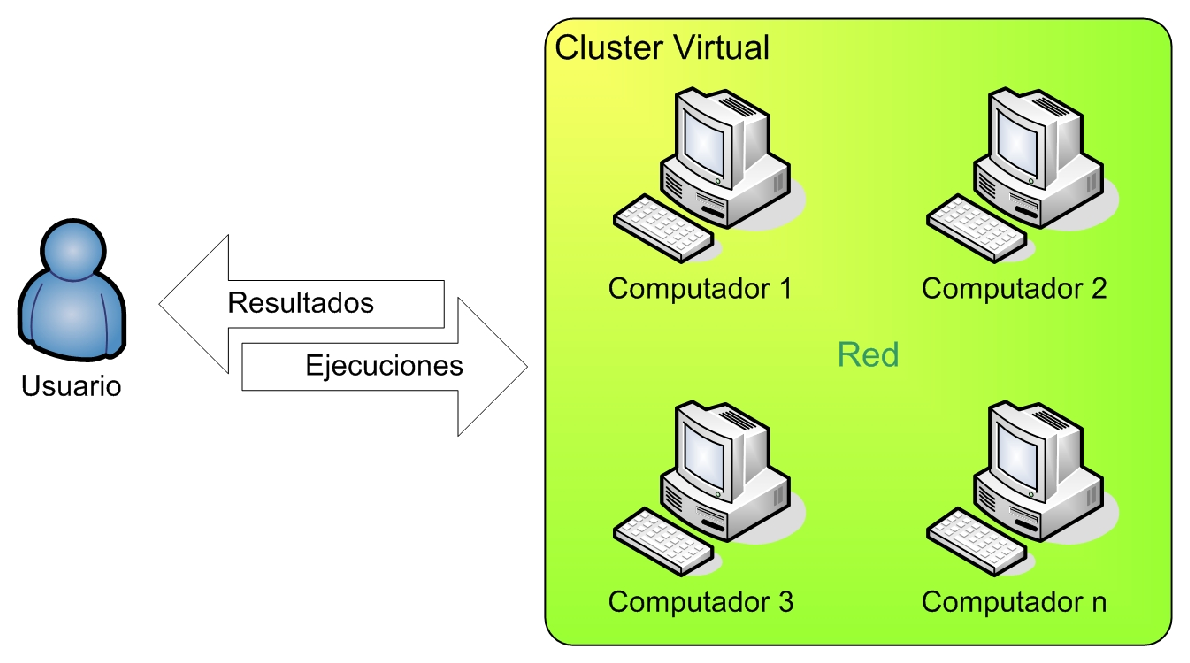
\includegraphics[width=0.7\textwidth]{images/image03.eps}
\end{center}
\caption{Esquema del sistema de cluster virtual}
\label{fig:image03}
\end{figure}
Para alcanzar los objetivos antes descritos se debe alcanzar una serie de etapas que comprenden los objetivos espec�ficos del proyecto. Los objetivos espec�ficos agrupados en sus respectivas etapas se describen a continuaci�n:
\paragraph{An�lisis bibliogr�fico}
Esta etapa consiste en un estudio sobre el tema de la computaci�n distribuida. Los objetivos de esta etapa son obtener antecedentes generales sobre el contexto del proyecto, describir los requerimientos del sistema y los recursos disponibles que hacen factible su implementaci�n, y analizar algunas de las soluciones existentes para establecer un punto base para el establecimiento de la arquitectura del proyecto.
\paragraph{Dise�o}
El objetivo de esta etapa es traducir los objetivos del proyecto en el dise�o de una soluci�n, en espec�fico, la arquitectura del sistema. En esta etapa se deben tratar los problemas l�gicos que surgen y las metodolog�as que permiten solucionarlos. 
\paragraph{Implementaci�n}
El objetivo de esta etapa es implementar la arquitectura del sistema en un software funcional. En esta etapa se deben tratar los problemas inherentes a la implementaci�n y la forma en que se abordan para darles soluci�n.
\paragraph{Evaluaci�n}
Los objetivos de esta etapa consisten en crear una aplicaci�n que utilice el sistema de cluster virtual y evaluar el rendimiento de �ste.
